% This file describes the general structure of some of our tb_dynamics models.

\section{Model Structure}

\subsection{General features}

We use a deterministic compartmental model including six types of compartments that represent 
different states of infection and disease of Tuberculosis (\emph{TB}). The model uses the same conceptual approach and similar 
assumptions to previously published models \cite{trauer-2017, ragonnet-2019, ragonnet-2021, ragonnet-2022}. 
Here we describe the model structure without treatment compartment and related factors (\emph{Figure \ref{fig:model}}). 
\newline
A susceptible compartment (S) is used to represent individuals who have 
never been infected with \emph{Mycobacterium tuberculosis (M.tb)}. Latent TB infection (LTBI) is modelled 
using two successive compartments: early latent (E) and late latent (L) to capture the declining risk of 
disease progression over time from infection \cite{ragonnet-2017}. The active disease compartment (I) represents 
individuals who have progressed to the active stage of TB disease. Diseased individuals who recover 
through self-cure progress directly to the recovered compartment (R).
\newline
Non-TB-related mortality is modelled by applying death rates to all model compartments. In addition, 
disease-specific mortality is implemented by applying increased mortality rates to the active disease 
compartments (I).
\newline
Reinfection occurs in the model in two different ways. First, latently infected individuals may be 
reinfected, with this process modelled using a flow from the late latent (L) to the early latent 
compartment (E). Second, individuals who have recovered from TB disease may be reinfected and 
return to the early latent compartment. The structure of our model allows for differential risk of 
infection for the currently and previously infected individuals, compared to the infection-naive 
individuals.
\begin{figure}[!htp]
    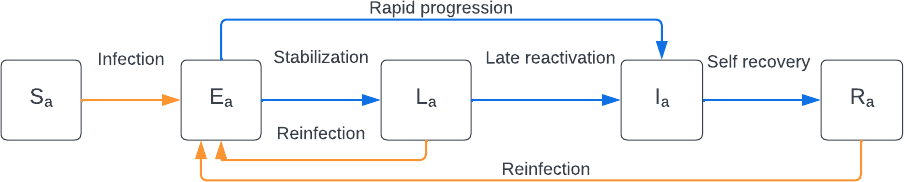
\includegraphics[width=\textwidth,height=\textheight,keepaspectratio]{images/model.png}
    \caption{Illustration of the model structure. 
    Boxes represent the different compartments types: susceptible (S), early latent (E), late latent (L), infectious (I), and recovered (R).
    The subscript indicates that compartments are stratified by age (a).}
    \label{fig:model}
\end{figure}

\subsection{Stratification by age}


The model is stratified using five categories: 0-4, 5-14, 15-34, 35-49 and 50+ years old. We assume 
heterogeneous mixing by age using an age-specific contact rate matrix. Since no local estimates of 
contact patterns by age were available for the Kiribati, we used a contact survey conducted in 
the Fijian population \cite{watson-2017} and adjusted the estimates to account for age distribution differences between
the two countries. Necessary age-stratified parameters for the basic model, including rate of stabilization from early to late latency,
rate of rapid progression to active TB, rate of late reactivation, relative risk of reinfection while latently infected, 
relative risk of reinfection after recovery were extracted from literature. Parameters are depicted in the Table \ref{tab:parameter}

